\chapter{L'eco nella caverna: perch\'{e} esiste la musica}

\begin{flushright}
	\textit{``La musica \`{e} la prova che la coscienza non \`{e} solo elaborazione di informazioni. \`{E} qualcosa di pi\`{u}. Qualcosa per cui non abbiamo ancora un nome.''}
\end{flushright}

\bigskip
\bigskip

Abbiamo attraversato i meccanismi del cervello umano, esaminato i suoi cortocircuiti cognitivi, catalogato i bias che ci condizionano. Abbiamo visto come la nostra mente sia un'architettura antica che opera con software moderno. Ma prima di chiudere questo viaggio, dobbiamo confrontarci con il mistero pi\`{u} inspiegabile che il nostro cervello produce: la musica.

Perch\'{e} esiste la musica? La domanda merita attenzione quanto il problema della coscienza. Eppure la diamo per scontata, come se fosse ovvio che la nostra specie dovesse sviluppare la capacit\`{a} di organizzare vibrazioni d'aria in sequenze che ci commuovono. Non lo \`{e} affatto.

Steven Pinker, in un momento di illuminata franchezza, l'ha definita piacere parassitario uditivo,\footnote{Pinker, S. (1997). \textit{How the Mind Works}. W. W. Norton and Company, New York.} una gratificazione che sfrutta circuiti cerebrali evoluti per altri scopi. Ma questa definizione, per quanto elegante, non rende giustizia al fenomeno. Un semplice piacere parassitario non sincronizza i battiti cardiaci di migliaia di persone in un concerto. Non resiste all'Alzheimer quando tutto il resto della memoria collassa. La musica \`{e} qualcosa di diverso da un semplice piacere parassitario.

\section{L'invenzione che nessuno ha inventato}

Cominciamo dal paradosso fondamentale: la musica non \`{e} stata inventata. Non c'\`{e} un Prometeo del suono che un giorno ha deciso di combinare ritmo e melodia per intrattenere la trib\`{u}. La musica \`{e} emersa, come emerge un mulinello nell'acqua quando le correnti si incontrano nel modo giusto. \`{E} il sottoprodotto accidentale di capacit\`{a} cognitive che si sono evolute per tutt'altri motivi.

Consideriamo il ritmo. Il nostro cervello riconosce pattern temporali perch\'{e} in natura significano sopravvivenza: il passo del predatore tra i cespugli, il battito nel grembo materno, la cadenza del camminare. Il nucleo caudato e il cervelletto,\footnote{Grahn, J. A., e Brett, M. (2007). Rhythm and beat perception in motor areas of the brain. \textit{Journal of Cognitive Neuroscience}, 19(5).} strutture antichissime, precedenti persino alla neocorteccia, erano gi\`{a} sintonizzati sui pattern ritmici molto prima che qualcuno decidesse di tamburellare su un tronco cavo.

Poi c'\`{e} il tono, la capacit\`{a} di distinguere le frequenze sonore. Anche questa non \`{e} nata per la musica, ma per decodificare le emozioni nella voce altrui. Un grugnito basso significa minaccia. Un tono acuto e tremolante significa paura. La prosodia emotiva,\footnote{Patel, A. D. (2008). \textit{Music, Language, and the Brain}. Oxford University Press, New York.} la melodia nascosta nel parlato, era gi\`{a} incorporata nel nostro sistema di comunicazione primordiale, quando ancora non avevamo parole ma solo suoni modulati.

\begin{center}
	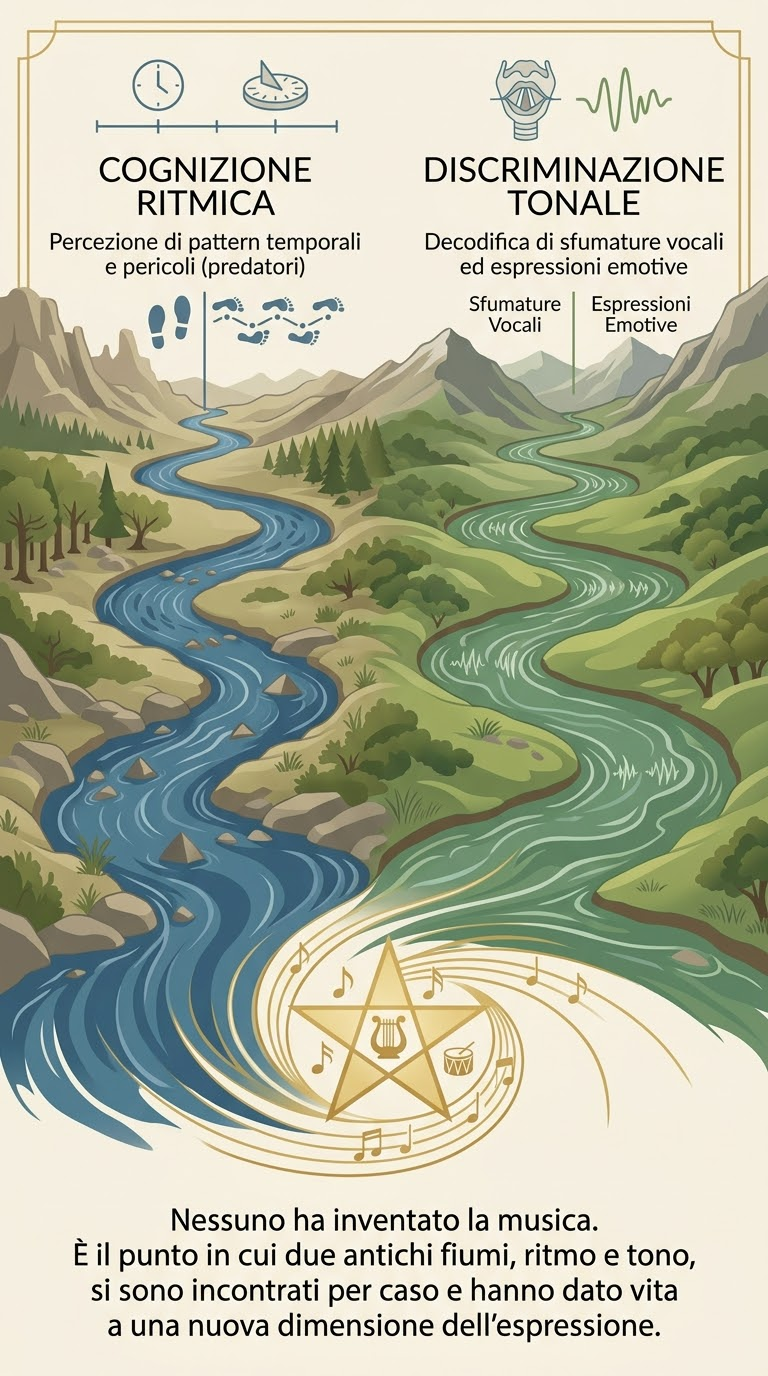
\includegraphics[width=0.8\textwidth]{images/musica_fusione_ritmo_tono.jpg}
	\captionof{figure}{La fusione accidentale da cui nasce la musica: il riconoscimento ritmico, evoluto per individuare pattern temporali di sopravvivenza, e la discriminazione tonale, evoluta per decodificare le emozioni nella voce, si incontrano come due fiumi che confluiscono per caso.}
	\label{fig:musica_fusione_ritmo_tono}
\end{center}

In qualche momento della nostra storia evolutiva, questi due sistemi, riconoscimento ritmico e discriminazione tonale, si sono incontrati. Non sappiamo esattamente quando. Forse gi\`{a} con \textit{Homo erectus}, attorno al fuoco, quando il battere di pietre contro pietre ha cominciato a seguire un pattern regolare. Forse con \textit{Homo heidelbergensis}, quando il controllo sempre pi\`{u} fine delle corde vocali ha permesso variazioni di tono intenzionali. Di certo sappiamo che \textit{Homo sapiens}, emerso circa 300.000 anni fa, aveva gi\`{a} questa capacit\`{a} pienamente sviluppata.

Quella fusione accidentale ha creato un dominio espressivo senza precedenti nel regno animale. Gli uccelli canori producono sequenze melodiche, \`{e} vero. Ma nessuna specie, eccetto noi, ha sviluppato la complessit\`{a} ritmica, melodica, armonica e timbrica della musica umana. Nessuna specie costruisce artefatti il cui unico scopo \`{e} produrre suoni organizzati. Oppure ce l'hanno?

\section{La colla invisibile della trib\`{u}}

Perch\'{e} se riflettiamo pi\`{u} attentamente, la musica ha un valore adattivo, solo che \`{e} molto pi\`{u} sottile di ``aiuta a cacciare'' o ``protegge dai predatori''. La musica \`{e} tecnologia sociale. \`{E} la colla invisibile che tiene insieme i gruppi umani.

Consideriamo un coro. Cosa succede neurologicamente quando decine di voci si fondono in un'unica linea melodica? I cervelli dei cantanti si stanno sincronizzando.\footnote{M\"uller, V., e Lindenberger, U. (2011). Cardiac and respiratory patterns synchronize between persons during choir singing. \textit{PLoS ONE}, 6(9).} Le loro onde cerebrali cominciano a pulsare all'unisono. I loro battiti cardiaci si allineano. I loro respiri convergono. Non \`{e} una metafora: \`{e} neurofisiologia documentata. Questa sincronizzazione ha un effetto psicologico profondo. Aumenta la fiducia reciproca. Amplifica l'empatia. Crea un senso di appartenenza che va oltre le parole. Dopo aver cantato insieme, le persone sono pi\`{u} disposte a cooperare, pi\`{u} generose, pi\`{u} propense a sacrificarsi per il gruppo.\footnote{Pearce, E., Launay, J., e Dunbar, R. I. M. (2015). The ice breaker effect: singing mediates fast social bonding. \textit{Royal Society Open Science}, 2(10).}

La musica \`{e} un collante tribale. E nella savana africana del Pleistocene, dove la trib\`{u} era tutto, l'unica difesa contro predatori, carestie, trib\`{u} rivali, un gruppo che cantava insieme era un gruppo che sopravviveva insieme. La selezione naturale, con la sua indifferente efficienza, ha favorito i gruppi musicali. Non perch\'{e} la musica in s\'{e} fosse utile, ma perch\'{e} rafforzava il legame sociale che era indispensabile.

Questa idea, che il canto tenga insieme un gruppo ancora prima che esistano parole compiute, non \`{e} soltanto una scoperta della biologia contemporanea. Nel 1781 Jean Jacques Rousseau, nel suo \textit{Saggio sull'origine delle lingue}, propose una tesi che al suo tempo sembr\`{o} eccentrica e che oggi riappare quasi identica nei laboratori di neuroscienze: il linguaggio umano, sosteneva, non nacque come prosa razionale, ma come canto.\footnote{Rousseau, J. J. (1781). \textit{Essai sur l'origine des langues}. Pubblicazione postuma, Ginevra.} Le prime parole, per Rousseau, non servivano a trasmettere informazioni pratiche, del tipo dov'\`{e} il cibo o attenzione al pericolo, ma a esprimere passioni, ed erano perci\`{o} pi\`{u} vicine a una melodia emotiva che a un enunciato logico. Solo in seguito, con la vita in societ\`{a} sempre pi\`{u} organizzate, il linguaggio si sarebbe progressivamente raffreddato in un sistema di segni astratti, perdendo per strada quella carica musicale originaria. Se Rousseau aveva ragione, la colla invisibile della trib\`{u} descritta sopra non \`{e} un uso secondario della musica, aggiunto in un secondo momento al linguaggio: \`{e} letteralmente la sua culla. Cantare insieme non sarebbe un modo particolare di comunicare, ma la forma pi\`{u} antica e pi\`{u} vera di comunicazione da cui tutte le altre, comprese le nostre parole pi\`{u} fredde e tecniche, sarebbero in seguito derivate.

Ma c'\`{e} un altro aspetto: la musica come esibizione sessuale. Qui entra in gioco il concetto di segnale costoso.\footnote{Zahavi, A., e Zahavi, A. (1997). \textit{The Handicap Principle}. Oxford University Press, Oxford.} In biologia evolutiva, un segnale \`{e} affidabile solo se \`{e} difficile da falsificare. Padroneggiare uno strumento richiede anni di pratica. Comporre una melodia originale richiede intelligenza, creativit\`{a}, controllo motorio fine. Un individuo musicalmente abile comunica efficienza cognitiva, salute fisica, disponibilit\`{a} di risorse da investire in attivit\`{a} non utilitaristiche. Geoffrey Miller ha sostenuto in modo convincente che molte delle nostre capacit\`{a} cognitive, linguaggio elaborato, senso dell'umorismo, creativit\`{a} artistica, si siano evolute principalmente come esibizioni sessuali,\footnote{Miller, G. (2000). \textit{The Mating Mind}. Doubleday, New York.} e la musica sarebbe la forma pi\`{u} pura e antica di questo fenomeno. \`{E} una forma di selezione sessuale, simile a quella che ha prodotto la coda del pavone. Anche le nostre espressioni pi\`{u} elevate affondano le radici nei meccanismi darwiniani di sopravvivenza e riproduzione. La musica non fa eccezione.

\section{La prima droga}

Ma se la musica fosse solo coesione sociale ed esibizione sessuale, sarebbe gi\`{a} abbastanza. Invece c'\`{e} qualcosa di pi\`{u} profondo. La musica \`{e} la prima tecnologia di alterazione della coscienza che la nostra specie ha sviluppato. Prima degli allucinogeni, prima dell'alcol, forse prima persino del fuoco. C'era il canto. E il canto altera letteralmente la chimica del cervello.

Cominciamo dal brivido musicale, quel momento di pura estasi quando una certa frase melodica, una progressione armonica particolare, ci attraversa come una scarica elettrica. Non \`{e} una metafora poetica: \`{e} un fenomeno misurabile, e coinvolge gli stessi circuiti neurochimici della morfina.\footnote{Salimpoor, V. N., e altri (2011). Anatomically distinct dopamine release during anticipation and experience of peak emotion to music. \textit{Nature Neuroscience}, 14(2).} Quando la musica raggiunge quel momento di climax emotivo, il nostro cervello rilascia endorfine,\footnote{Chanda, M. L., e Levitin, D. J. (2013). The neurochemistry of music. \textit{Trends in Cognitive Sciences}, 17(4).} oppioidi endogeni, chimicamente simili alla morfina. Non stiamo usando una metafora quando diciamo che la musica ci droga: ci stiamo letteralmente drogando con frequenze sonore organizzate.

Molto prima che la neurochimica potesse dimostrarlo con uno scanner, un filosofo tedesco aveva gi\`{a} intuito che la musica agisse su di noi in modo radicalmente diverso da ogni altra arte. Arthur Schopenhauer, ne \textit{Il mondo come volont\`{a} e rappresentazione}, sostenne che tutte le altre arti, la pittura, la scultura, persino la poesia, ci parlano attraverso rappresentazioni: ci mostrano un'immagine del mondo, un oggetto, un'idea.\footnote{Schopenhauer, A. (1818). \textit{Die Welt als Wille und Vorstellung}. Brockhaus, Lipsia.} La musica, invece, per Schopenhauer non rappresenta nulla: non \`{e} un'immagine della realt\`{a}, ma la voce diretta di ci\`{o} che lui chiamava la Volont\`{a}, quella forza cieca e incessante che secondo lui pulsa dietro ogni fenomeno del mondo, dal desiderio pi\`{u} elementare fino al pi\`{u} astratto pensiero. Per questo, scriveva, la musica ci commuove con una forza che nessun'altra arte possiede: mentre un quadro ci parla del mondo, la musica \`{e} il mondo, còlto per un istante nella sua pulsazione pi\`{u} intima, prima ancora di trasformarsi in immagine o concetto. \`{E} la stessa intuizione, spogliata del linguaggio metafisico ottocentesco, che ritroviamo nella scoperta che la musica condivide i circuiti della morfina: se davvero ci parla senza la mediazione di alcuna immagine, ha senso che ci raggiunga tanto in profondit\`{a} da alterare la chimica stessa del cervello, come nessuna rappresentazione potrebbe mai fare.

\section{Il cervello accordato}

Se la musica fosse davvero solo un sottoprodotto accidentale, dovremmo trovare nel cervello un'area dedicata al suo processamento, un modulo musicale, analogamente a come abbiamo un'area di Broca per il linguaggio. Invece troviamo qualcosa di molto pi\`{u} strano. La musica non ha una sede specifica nel cervello. Quando ascoltiamo musica, si attiva una rete di aree cerebrali pi\`{u} vasta di quella richiesta dalla maggior parte degli altri compiti cognitivi.\footnote{Levitin, D. J., e Tirovolas, A. K. (2009). Current advances in the cognitive neuroscience of music. \textit{Annals of the New York Academy of Sciences}, 1156.} La corteccia uditiva primaria per processare le frequenze, il cervelletto e i gangli della base per il ritmo, la corteccia prefrontale per la sintassi musicale, l'ippocampo per la memoria, l'amigdala per le emozioni.

\`{E} come se la musica, invece di essere un'applicazione installata in una zona specifica del cervello, fosse un sistema operativo che pervade l'intera architettura neurale. Una delle conseguenze pi\`{u} evidenti \`{e} la resilienza anomala della memoria musicale. Oliver Sacks, in \textit{Musicophilia},\footnote{Sacks, O. (2007). \textit{Musicophilia: Tales of Music and the Brain}. Alfred A. Knopf, New York.} documenta pazienti con Alzheimer avanzato che non riconoscono pi\`{u} i propri figli ma possono ancora cantare le canzoni della loro giovinezza, parola per parola. La memoria musicale resiste quando altre forme di memoria collassano, probabilmente proprio per la sua natura distribuita: non \`{e} memorizzata in un punto, ma diffusa attraverso la rete, e la rete, anche danneggiata, cerca di ricostruirla.

\begin{center}
	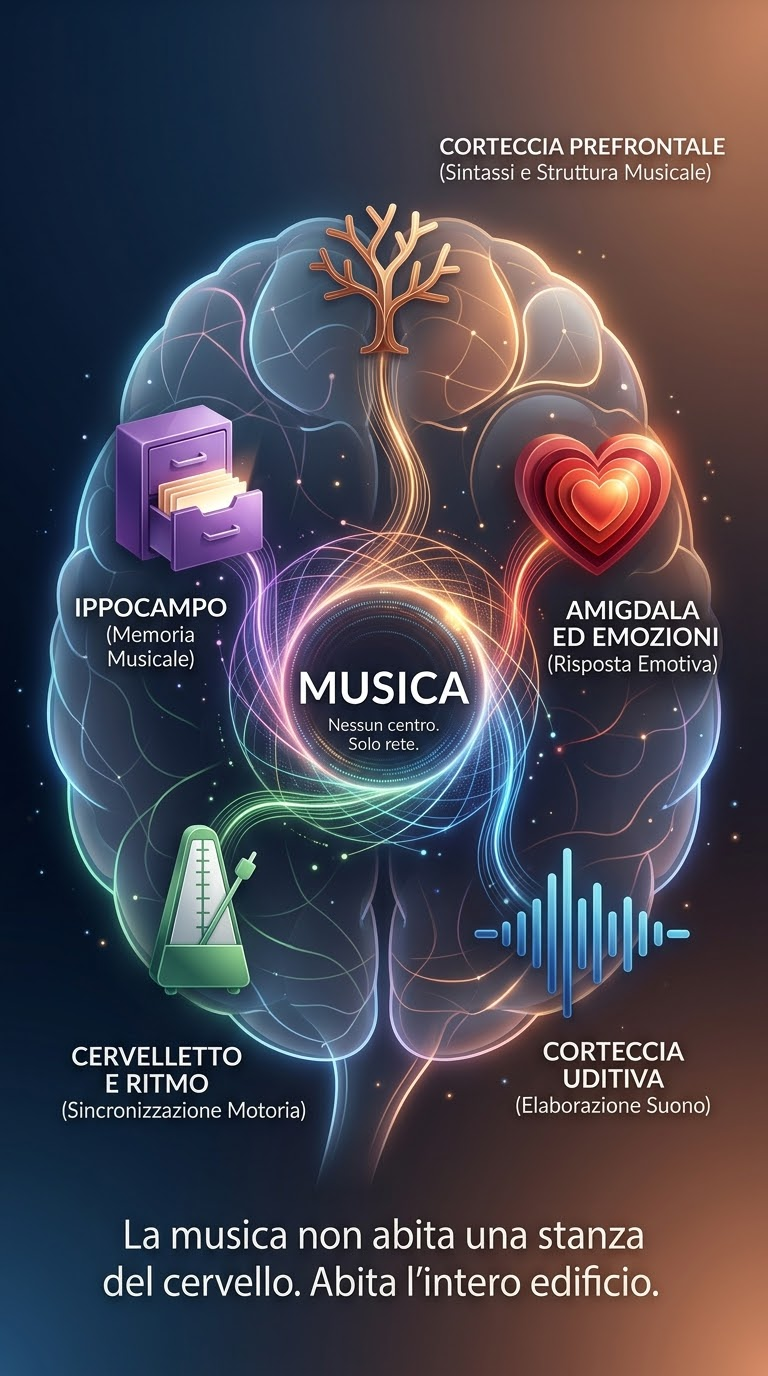
\includegraphics[width=0.8\textwidth]{images/1000093151.jpg}
	\captionof{figure}{La distinzione di Schopenhauer: mentre le altre arti rappresentano il mondo attraverso un'immagine, la musica \`{e}, secondo il filosofo, la voce diretta della Volont\`{a} che pulsa dietro ogni fenomeno.}
	\label{fig:musica_schopenhauer_volonta}
\end{center}


Poi c'\`{e} il mistero dell'orecchio assoluto.\footnote{Zatorre, R. J. (2003). Absolute pitch: A model for understanding the influence of genes and development on neural and cognitive function. \textit{Nature Neuroscience}, 6(7).} Solo circa una persona su diecimila possiede questa capacit\`{a}: riconoscere e nominare una nota musicale senza alcun riferimento esterno. L'aspetto interessante \`{e} che tutti i neonati sembrano possederla, ma la maggior parte la perde nei primi anni di vita, come se la nostra cultura ci disimparasse questa capacit\`{a}. Impariamo a pensare in termini relativi, questa nota \`{e} pi\`{u} alta di quella, e nel processo perdiamo la capacit\`{a} di percepirle in modo assoluto.

E poi c'\`{e} il legame profondo tra musica e matematica. I pitagorici lo avevano intuito duemilacinquecento anni fa: i rapporti armonici sono rapporti numerici. Un'ottava corrisponde a un rapporto di frequenze due a uno, una quinta perfetta a tre a due. Ma non \`{e} solo questione di rapporti tra note. La struttura stessa della composizione musicale, le fughe di Bach, obbedisce a principi matematici profondi. Una fuga \`{e} essenzialmente un teorema musicale: prendi un tema, applicagli trasformazioni secondo regole precise, e vedi cosa emerge. Il risultato non \`{e} solo corretto matematicamente, \`{e} bello. C'\`{e} un substrato cognitivo comune, probabilmente legato alla capacit\`{a} di costruire rappresentazioni gerarchiche, che permette sia la musica che la matematica, e in ultima analisi la coscienza stessa. Forse arte e scienza non sono magisteri separati: sono due manifestazioni diverse della stessa capacit\`{a} cognitiva fondamentale, trovare ordine nel caos, pattern nel rumore, bellezza nella struttura.

\section{Il vaccino emotivo}

Ma veniamo ora a un paradosso interessante: perch\'{e} amiamo la musica triste? Dal punto di vista evolutivo, dovremmo evitare ci\`{o} che ci causa sofferenza. Eppure cerchiamo attivamente musica che ci fa piangere, che evoca malinconia, nostalgia, perdita.

Una possibile spiegazione viene dalla teoria della palestra emotiva.\footnote{Huron, D. (2006). \textit{Sweet Anticipation: Music and the Psychology of Expectation}. MIT Press, Cambridge.} La musica triste ci permette di praticare la sofferenza in un ambiente sicuro. \`{E} un vaccino emotivo: ci inoculiamo dosi controllate di tristezza per costruire anticorpi contro quella reale. Quando ascoltiamo una ballata straziante sappiamo, a livello conscio, che non stiamo davvero subendo una perdita. Ma a livello emotivo, quello delle strutture limbiche profonde che non capiscono la differenza tra reale e simulato, la sofferenza \`{e} autentica. E quindi impariamo che la tristezza, per quanto dolorosa, \`{e} sopportabile, che ha una struttura, un inizio e una fine, che possiamo attraversarla e uscirne dall'altra parte.

Gli studi neurobiologici supportano questa interpretazione. Quando ascoltiamo musica triste, il cervello rilascia prolattina,\footnote{Huron, D. (2011). Why is sad music pleasurable? A possible role for prolactin. \textit{Musicae Scientiae}, 15(2).} lo stesso ormone rilasciato durante l'allattamento, associato a consolazione e legame sociale. Ci stiamo letteralmente consolando da soli, attraverso la mediazione della musica. E c'\`{e} un'altra dimensione: la musica triste \`{e} bella. C'\`{e} qualcosa di esteticamente perfetto in una melodia malinconica ben costruita, quello che i giapponesi chiamano \textit{mono no aware}, la consapevolezza acuta e toccante della transitoriet\`{a} delle cose. La musica triste ci insegna che la sofferenza pu\`{o} essere trasformata in bellezza. Non elimina la sofferenza, ma le d\`{a} forma, struttura, significato.

\section{Il silenzio, la macchina e l'ultima domanda}

Miles Davis, genio del jazz e maestro dell'economia espressiva, disse una volta che la musica non sta nelle note, ma nel silenzio tra le note.\footnote{Davis, M., citato in Carr, I. (1982). \textit{Miles Davis: A Biography}. William Morrow, New York.} \`{E} una frase che suona poetica, quasi mistica, ma contiene una verit\`{a} cognitiva profonda. Il silenzio nella musica non \`{e} assenza: \`{e} presenza negativa, uno spazio che il cervello riempie con anticipazione, con memoria, con aspettativa.

Ma quali suoni il nostro cervello \`{e} davvero calibrato per ascoltare? Per 300.000 anni il paesaggio sonoro umano era radicalmente diverso: vento tra le foglie, acqua corrente, canto degli uccelli secondo pattern prevedibili. Il sistema nervoso si \`{e} ottimizzato su questi suoni come condizione di normalit\`{a}.\footnote{Bratman, G. N., e altri (2015). Nature experience reduces rumination and subgenual prefrontal cortex activation. \textit{Proceedings of the National Academy of Sciences}, 112(28).} Il rumore moderno, traffico, notifiche, macchinari, \`{e} neurologicamente ostile: frequenze irregolari, volume imprevedibile, pattern che il cervello non pu\`{o} abituarsi a processare completamente. La verit\`{a} \`{e} che non ti rilassi con i suoni naturali. Ti stressi senza di loro. E forse \`{e} proprio in questo scarto, tra il paesaggio sonoro per cui siamo calibrati e quello in cui viviamo, che si nasconde una delle ragioni del nostro bisogno di musica: un tentativo di ricostruire, artificialmente, una struttura sonora che il cervello possa riconoscere come familiare.

Questa natura relazionale della percezione sonora solleva una domanda interessante nell'era dell'intelligenza artificiale musicale. Possiamo descrivere perfettamente i meccanismi. Sappiamo quali aree cerebrali si attivano. Conosciamo i neurotrasmettitori coinvolti. Un'intelligenza artificiale sufficientemente sofisticata potrebbe fare tutto questo, e molto di pi\`{u}, con una precisione che nessun musicologo umano potrebbe eguagliare. Ma quell'intelligenza artificiale sentirebbe qualcosa ascoltando una sinfonia di Mahler? Avrebbe i brividi lungo la schiena quando la progressione armonica raggiunge quel punto di perfetta risoluzione?

Suno AI, lanciata nel 2023, pu\`{o} generare in pochi secondi una canzone completa, voce, strumenti, struttura, emozioni, partendo da una semplice descrizione testuale.\footnote{Suno, Inc. (2024). Documentazione della piattaforma. Cambridge, Massachusetts.} Il paradosso \`{e} evidente: un algoritmo che non ha mai provato gioia pu\`{o} comporre una melodia gioiosa. Come \`{e} possibile? Suno ha ingerito milioni di canzoni umane. Ha estratto pattern, strutture, progressioni armoniche. \`{E} mimesi computazionale pura: la macchina che impara a imitare i gesti emotivi senza provare l'emozione.

Per capire meglio cosa manchi esattamente a quella mimesi, aiuta tornare a un secondo pensatore tedesco, allievo insofferente proprio di Schopenhauer. Nel 1872 Friedrich Nietzsche, ne \textit{La nascita della tragedia}, distinse due forze opposte e complementari nell'arte greca.\footnote{Nietzsche, F. (1872). \textit{Die Geburt der Trag\"odie}. E. W. Fritzsch, Lipsia.} \textit{L'apollineo} \`{e} il principio della forma, dell'ordine, del sogno lucido, dell'individuo ben distinto dagli altri: \`{e} la scultura, l'architettura, l'immagine chiara. Il \textit{dionisiaco}, invece, \`{e} il principio dell'ebbrezza, della fusione, della perdita temporanea dei confini dell'io in qualcosa di pi\`{u} grande, ed \`{e}, per Nietzsche, il territorio proprio della musica. Quando cantiamo insieme in un coro, quando un intero pubblico si muove all'unisono a un concerto, non stiamo semplicemente ascoltando una forma ben costruita: stiamo attraversando, per qualche istante, quella dissoluzione dionisiaca del confine tra s\'{e} e gli altri che Nietzsche considerava l'esperienza estetica pi\`{u} radicale possibile. Ed \`{e} qui che il limite della musica generata da una macchina diventa filosoficamente nitido: un algoritmo pu\`{o} produrre perfettamente la forma apollinea, la struttura, l'armonia corretta, la progressione attesa, ma non ha nulla dentro di s\'{e} da dissolvere. Genera l'apollineo che imita il dionisiaco: superficie senza abisso, la forma dell'ebbrezza senza l'ebbrezza stessa, perch\'{e} non esiste alcun confine dell'io, in una macchina, che possa mai essere davvero perduto.

Studi recenti sembrano confermare questo scarto anche a livello fisiologico. Il nostro cervello reagisce in modo sottilmente diverso alla musica generata dall'intelligenza artificiale rispetto a quella composta da umani, anche quando non sappiamo quale stiamo ascoltando.\footnote{Fi\v{s}er, N., e altri (2025). Emotional impact of AI generated vs. human composed music. \textit{PLOS One}, 20(1).} Le pupille si dilatano di pi\`{u} con la musica generata dall'intelligenza artificiale, segno di maggiore sforzo cognitivo, mentre la risposta galvanica della pelle indica livelli di attivazione pi\`{u} bassi. Eppure, e qui sta il vero mistero, l'impatto emotivo soggettivo \`{e} quasi identico: le persone riportano le stesse emozioni ascoltando musica generata da una macchina o da un essere umano. \`{E} come se l'emozione musicale potesse essere replicata con precisione algoritmica, ma il corpo, nella sua saggezza animale, mantenesse comunque una traccia della differenza.

C'\`{e} forse un modo pi\`{u} preciso per nominare quella traccia sottile che il corpo percepisce e la mente cosciente no. Negli anni Quaranta la filosofa americana Susanne Langer, in \textit{Filosofia in una nuova chiave}, propose una distinzione decisiva tra due modi in cui un segno pu\`{o} riferirsi a un significato.\footnote{Langer, S. K. (1942). \textit{Philosophy in a New Key}. Harvard University Press, Cambridge.} Un segno discorsivo, come una parola, descrive un'emozione dall'esterno, la nomina, la classifica in una categoria gi\`{a} pronta: la parola tristezza non \`{e} triste, ne \`{e} soltanto l'etichetta. La musica, per Langer, funziona in modo del tutto diverso: \`{e} un simbolo presentativo, che non descrive l'esperienza emotiva ma ne presenta direttamente la forma logica, la stessa struttura dinamica di tensione e distensione che caratterizza il sentire umano. Ecco perch\'{e}, secondo Langer, la musica riesce a comunicare sfumature emotive per cui nessuna parola esiste: non le sta descrivendo dall'esterno, ne sta incarnando la forma stessa. E questo spiega, forse meglio di ogni altra teoria, perch\'{e} la musica generata da una macchina possa suonarci sottilmente vuota anche quando tecnicamente perfetta: pu\`{o} copiare con esattezza la forma del simbolo, la sequenza di tensioni e risoluzioni che Langer descriveva, senza per\`{o} che dietro quella forma vi sia mai stata una reale esperienza emotiva da presentare. Non manca la superficie. Manca ci\`{o} di cui la superficie, in un compositore umano, \`{e} sempre stata l'impronta diretta.

E qui sorge la domanda: se l'intelligenza artificiale pu\`{o} generare musica che fa risuonare i nostri cervelli allo stesso modo, stiamo forse permettendo alle macchine di riprogrammare i nostri stati di coscienza? La risposta non \`{e} ancora scritta. Ma una cosa \`{e} certa: stiamo rinegoziando il contratto pi\`{u} antico della nostra specie, quello tra la mente che crea e il mistero da cui la creazione emerge.

L'algoritmo continua a generare musica. Senza gioia, senza dolore, senza sapere cosa significhi cantare. Eppure produce suoni che ci commuovono. \`{E} qui che la musica diventa una sonda filosofica potente quanto il problema della stanza cinese di Searle o lo zombie filosofico di Chalmers.\footnote{Chalmers, D. J. (1996). \textit{The Conscious Mind}. Oxford University Press, New York.} Perch\'{e} se un sistema pu\`{o} processare perfettamente tutte le informazioni musicali ma non sentire nulla, allora manca qualcosa di fondamentale, qualcosa che non \`{e} riducibile al processamento di informazioni. Qualcosa che Thomas Nagel chiamava com'\`{e} essere,\footnote{Nagel, T. (1974). What is it like to be a bat? \textit{The Philosophical Review}, 83(4).} la qualit\`{a} soggettiva dell'esperienza.

La musica, in altre parole, \`{e} la prova vivente, o meglio udibile, che la coscienza \`{e} pi\`{u} della somma delle sue parti computazionali. Forse la domanda giusta non \`{e} perch\'{e} esiste la musica, ma cosa ci dice la musica sull'universo. Perch\'{e} se pattern sonori organizzati possono produrre emozioni profonde, se il silenzio tra le note pu\`{o} essere denso di significato quanto le note stesse, allora forse l'universo \`{e} strutturato in modo da permettere, o addirittura favorire, l'emergere di fenomeni come la coscienza e l'esperienza soggettiva.

La musica non risolve il problema difficile della coscienza. Ma ce lo ricorda, ogni volta che ascoltiamo. Ci ricorda che essere consapevoli non \`{e} solo elaborare informazioni. \`{E} essere qualcosa. \`{E} avere un punto di vista sul mondo. \`{E} trasformare input sensoriali in esperienza vissuta. E finch\'{e} una macchina, per quanto sofisticata, non potr\`{a} dirci cosa significhi davvero ascoltare il \textit{Requiem} di Mozart, non descriverlo ma viverlo, sapremo che c'\`{e} ancora un abisso tra il processamento e la coscienza.

La musica non \`{e} nelle note. Ma se non \`{e} nelle note, e non \`{e} nemmeno necessariamente nell'umano che le organizza, allora dove risiede? Nel cervello che ascolta? Nell'interazione tra suono e percezione? O in quella zona ancora inesplorata dove computazione ed esperienza soggettiva si incontrano? Un abisso del silenzio tra le note. Un abisso che solo la musica, forse, pu\`{o} farci percepire nella sua profondit\`{a}.